
\documentclass[a4paper,12pt]{article}

\usepackage{url}
\usepackage{graphicx}

\title{PeerSim HOWTO 2: build a topology generator}

\author{Gian Paolo Jesi (jesi@cs.unibo.it)}

\begin{document}

\maketitle

\section{Introduction}

This tutorial teaches you how to build from scratch a new peersim
( peersim project page: \url{http://sourceforge.net/projects/peersim}
) topology generator. In order to understand this tutorial, the reader
is encouraged to start reading the first peersim tutorial 
(\url{http://peersim. sourceforge.net/peersim_HOWTO.html}) 
to have an idea of the basic concepts that will not be discussed any
further in this document. 

The aim of this tutorial is to be as practical as possible; the goal
is to give the reader ideas about technical or intermediate level
features of peersim and to encourage him/her to experiment further.
The full source code discussed in this document is available via CVS
at peersim project page in the \emph{peersim.example.hot} class package.


\section{What is a topology?}

The network abstraction in peersim is a (sometimes huge) array of
\emph{Node} structures (interfaces); because of the size of the network
and to overcome scalability problems, usually in large P2P networks
each node knows about the existence of a very small subset of other
nodes (ex: order of $\log(N)$ where $N$ is the whole network size). Thus
each node has a short list of other node references, usually called
``neighbors'', build accordingly to some kind of strategy
or rule. 

Thus, we can say that a topology is how nodes are arranged (linked)
together and clearly this depends upon the particular chosen rule.
Examples of topology are the following (not exhaustive at all): 

\begin{itemize}
\item random graphs 
\item Watts-Strogatz model graph 
\item star model 
\item ring model 
\item lattice model 
\item ...
\end{itemize}

\subsection{Which rule to choose?}
\label{sec:rule}

In this document, we have chosen to code a particular topology generator
to build Internet-like tree topologies. The building process is based
on the \emph{preferential attachment} approach. The rule applied is
quite simple and takes into account geometric and network constraints
to better mimic real world network. The preferential attachment choice
can be affected by a parameter ($ \alpha $) that amplifies or reduces the
geometric location influence in favor of the path distance. 

The rule strategy is the following: we consider a square unit region
$D$, then we start with node $x(0)$ chosen at random and we set $W(x(0))
= 0$ (it i

s the root node). For each i with $i = 1...n-1$ we choose a
new node $x(i)$ in the region $D$ and we connect it to an \textbf{early
inserted} node $x(j)$ that minimize the following formula:

\begin{center}
$W(x(j)) + \alpha \cdot dist(x(i), x(j))$ with 0 $\leq$ j $<$ i
\end{center}

where: 

\begin{itemize}
\item $W(x(j))$ is the distance in terms of hops (the path distance from node
$x(j)$ to the root node); 
\item $dist(...)$ is the usual Euclidean distance; 
\item $ \alpha $ is a weight parameter that can minimize or maximize 
the geometric distance influence;
 
\end{itemize}

After having chosen a node $x(j)$, we set $W(x(i)) = W(x(j))+1$ . At
the end we obtain a tree rooted in $x(0)$.

We have extended this model to improve robustness allowing every node
to have exactly $d$ outbound neighbors instead of only one. This means
that, at the time of joining the network, each node should have at
least $d$ candidates to be selected as neighbors. To achieve this property,
as a first step we select at random exactly $d$ root nodes and we connect
them together in a ring fashion (a doubly linked list). In this way
each ordinary node has at least $d$ nodes (the $d$ roots) to choose from
in order to select its neighbors. In other words, each node has to
select the best $d$ nodes that minimize the function above. 

To get further details about this model, we suggest the following
readings:

\begin{enumerate}

\item ``Heuristically Optimized Trade-offs: A New Paradigm for Power
Laws in the Internet'' \\
(\url{http://cgi.di.uoa.gr/~elias/publications/paper-fkp02.pdf} )

\item  ``Degree distributions
of the FKP network model'' \\
(\url{http://research.microsoft.com/~jchayes/Papers/FKPdgrees.pdf}) 

\item ``On Power-Law
Relationships of the Internet Topology''\\
(\url{http://www.cs.ucr.edu/~michalis/CAMERA.ps})

\end{enumerate}

The model should generate a topology that exhibits a power-law bound
on the in-degree sequence of nodes; but, as stated in the second
previously listed paper, this power-law prediction is not true.

\section{What we need to code}

Our aim is to have a component able to produce the desired topology
according to the $\alpha$ and $d$ parameters. We are not interested
in building the topology in a set of steps over time: we want
something like an initializer that arranges the wiring from scratch in
one step.

In order to obtain this behavior, we need to write the following
Java classes:  

\begin{itemize}

\item the protocol class: the protocol itself does nothing because 
we want something that auto-magically builds this topology model from 
a raw list of unconnected nodes. This class is a sort of structure to
collect some needed values, such as the node space coordinates, the
hop distance, the in-degree counter and so on.  
The reader can think to this class as ``glue code''.
 
\item a \emph{Control} class to initialize coordinates and to wire nodes
  according to the rules described in Section~\ref{sec:rule}. The
  wiring mechanism is based on a peersim feature
  (\emph{peersim.dynamics.WireByMethod} class) that makes the creation of
  factories out of any static method, a straightforward
  process. However we can consider this component as the topology
  factory class. 

\item a \emph{Control} to monitor and collect statistics about the
  generated topology. It has to to print to file the coordinates (in
  order to visualize the topology) and to collect statistics about the
  in-degree distribution.

\end{itemize}

\section{Code writing}

\subsection{Protocol class}

As we stated so far, the protocol code is minimal:

\footnotesize
\begin{verbatim}
 import peersim.core.IdleProtocol;
 
 public class InetNodeProtocol extends IdleProtocol {
     // coordinates in space:
     public double x;
     public double y;
     
     public int in_degree;
     public int hops;
     public boolean isroot;
    
     /** Creates a new instance of hotNodeProtocol */
     public InetNodeProtocol(String prefix, Object obj) {
    super(prefix);
         in_degree = 0;
         hops = 0;
         isroot = false;
     }
     
     public Object clone() throws CloneNotSupportedException {
         InetNodeProtocol af = (InetNodeProtocol) super.clone();
         ...
         return af;
     }
    
     public void nextCycle(peersim.core.Node, int protocolID) {
     }

\end{verbatim}
\normalsize

The \emph{nextCycle()} method is empty, so it is presence is completely 
optional. The class is basically a structure encapsulated in an
object. Another solution could be to define a specialized sub-class of
\emph{peersim.core.GeneralNode} in which the variables can be stored
and then use \emph{peersim.core.IdleProtocol} to handle the nodes
``who knows whom'' relations. Both the approaches are identical in
practice, it is just a developer choice. The reader can implement this
second suggestion just for exercise.


\subsection{The factory class}

The factory first work is to initialize the structure hold in the
protocol class. Basically, it has to assign random coordinates to
nodes, to reset the hop count and to mark nodes as non-root.

From the outside (means from the peersim configuration file) only two 
main parameters are required: the \emph{Linkable} enabled protocol to
initialize and the outbound degree $d$. the $\alpha$ parameter is
handled elsewhere, we will see later how and where it is managed. 
The constructor method 
takes care of collecting these parameters or to set up the corresponding 
default values.

\footnotesize
\begin{verbatim}
public class InetInitializer implements Control {
     /** 
      * String name of the parameter that defines the protocol to initialize.
     * Parameter read will has the full name
     * <tt>prefix+"."+PAR_PROT</tt>
     */
     public static final String PAR_PROT = "protocol";
 
     /**
      * String name of the parameter about the out degree value.
     */
     public static final String PAR_OUTDEGREE = "d";
     
     /**
      * String name of the parameter used as a maximum x or y coordinate. All the 
      * nodes are on a square region.
     */
     public static final String PAR_MAX_COORD = "max_coord";
    
     ....
     
     /** Creates a new instance of InetInitializer */
     public InetInitializer(String prefix) {
         // super(prefix);
         pid = Configuration.getPid(prefix+"."+PAR_PROT);
         d = Configuration.getInt(prefix+"."+PAR_OUTDEGREE);
         
         maxcoord = Configuration.getDouble(prefix + "." + PAR_MAX_COORD, 1.0);
     }
}
\end{verbatim}
\normalsize
     
The class implements the \emph{Control} interface and thus the
\emph{execute()} method is mandatory. Here, the actual node initialization
is performed.

The next step regards the tree root(s) election. If there is only a
single root, its coordinates are centered in the square (default edge
size: 1.0), otherwise
random coordinates are assigned (as for any ordinary node).

\footnotesize 
\begin{verbatim}
 public boolean execute() {
        Random rnd = CommonState.r;
        System.out.println(DEBUG_STRING + "size: " + Network.size()
                + " outdegree: " + d);

        // build outdegree roots
        System.out.println(DEBUG_STRING + "Generating " + d
                + " root(s), means out degree " + d + "...");
        for (int i = 0; i < d; ++i) {
            Node n = (Node) Network.get(i);
            InetNodeProtocol prot = (InetNodeProtocol) n.getProtocol(pid);
            prot.isroot = true;
            prot.hops = 0;
            prot.in_degree = 0;
            if (d == 1) {
                prot.x = maxcoord / 2;
                prot.y = maxcoord / 2;
            } else { // more than one root
                if (rnd.nextBoolean()) {
                    prot.x = maxcoord / 2 + (rnd.nextDouble() * 0.1);
                } else {
                    prot.x = maxcoord / 2 - (rnd.nextDouble() * 0.1);
                }
                if (rnd.nextBoolean()) {
                    prot.y = maxcoord / 2 + (rnd.nextDouble() * 0.1);
                } else {
                    prot.y = maxcoord / 2 - (rnd.nextDouble() * 0.1);
                }
                System.out.println("root coord: " + prot.x + " " + prot.y);
            }
        }

        // Set coordinates x,y and set indegree 0
        System.out.println(DEBUG_STRING
                + "Generating random cordinates for nodes...");
        for (int i = d; i < Network.size(); i++) {
            Node n = (Node) Network.get(i);
            InetNodeProtocol prot = (InetNodeProtocol) n.getProtocol(pid);
            if (maxcoord == 1.0) {
                prot.x = rnd.nextDouble();
                prot.y = rnd.nextDouble();
            } else {
                prot.x = rnd.nextInt((int) maxcoord);
                prot.y = rnd.nextInt((int) maxcoord);
            }
            prot.in_degree = 0;
        }
        return false;
    }
\end{verbatim}
\normalsize

The actual factory is responsible of the wiring process. The factory pattern
is obtained using the \emph{peersim.dynamics.WireByMethod} class. This
peersim feature allows to specify, in the config file, a class to be used
as an \emph{indirect factory} and one of its method. The specified
method has some constraints: it has to be static and its first
argument must be a \emph{Graph} type. The \emph{Graph} interface is
very useful in peersim because it let the developer to access to the node
topology with a graph-like abstraction and to apply graph algorithms
(many algorithms can be found in \emph{peersim.graphGraphAlgorithms}
class).

Other parameters can be declared for the static method with the
parameter \texttt{arg} followed by a index number starting from 1 (the
argument 0 is by default the graph object). A working setup can be
the following:

\footnotesize
\begin{verbatim}
init.1 WireByMethod
init.1.class example.hot.InetInitializer
init.1.method wireHOTOverlay
init.1.arg1 2 # d
init.1.arg2 0.5 # alfa , default 0.5 
\end{verbatim}
\normalsize

Our class implements the actual factory method in
\emph{wireHOTOverlay()}, however by default \emph{WireByMethod} invokes
a plain \emph{wire()} method (that is also present and simply calls
our specialized one). The parameters are the degree $d$
and the $\alpha$ value. Here, in fact, is where the $\alpha$ parameter
come into play.

If there are more than one root node, the factory  
joins them together in a ring (connections are non oriented). As an exercise, 
the reader can change this choice implementing something else (ex: putting 
the root nodes in a fully connected topology or a random graph or
whatever).

Then, the wiring process does the following: for each node $n$ other than
root(s), it takes exactly $d$ nodes that minimizes the formula (see
Section \ref{sec:rule} and connects node $n$ those $d$ nodes.

\footnotesize
\begin{verbatim}
public static void wireHOTOverlay(Graph g, int outDegree, double alfa) {
        // Connect the roots in a ring if needed (thus, if there are more than 1
        // root nodes.
        if (outDegree > 1) {
            System.out.println(DEBUG_STRING + "Putting roots in a ring...");
            for (int i = 0; i < outDegree; i++) {
                Node n = (Node) g.getNode(i);
                ((InetNodeProtocol) n.getProtocol(pid)).in_degree++;
                n = (Node) g.getNode(i + 1);
                ((InetNodeProtocol) n.getProtocol(pid)).in_degree++;

                g.setEdge(i, i + 1);
                g.setEdge(i + 1, i);
            }
            Node n = (Node) g.getNode(0);
            ((InetNodeProtocol) n.getProtocol(pid)).in_degree++;
            n = (Node) g.getNode(outDegree);
            ((InetNodeProtocol) n.getProtocol(pid)).in_degree++;
            g.setEdge(0, outDegree);
            g.setEdge(outDegree, 0);
        }

        // for all the nodes other than root(s), connect them!
        for (int i = outDegree; i < Network.size(); ++i) {
            Node n = (Node) g.getNode(i);
            InetNodeProtocol prot = (InetNodeProtocol) n.getProtocol(pid);

            prot.isroot = false;

            Node candidate = null;
            int candidate_index = 0;
            double min = Double.POSITIVE_INFINITY;
            if (outDegree > 1) {
                int candidates[] = getParents(g, pid, i, outDegree, alfa);
                for (int s = 0; s < candidates.length; s++) {
                    g.setEdge(i, candidates[s]);
                    Node nd = (Node) g.getNode(candidates[s]);
                    InetNodeProtocol prot_parent = (InetNodeProtocol) nd
                            .getProtocol(pid);
                    prot_parent.in_degree++;
                }
                // sets hop
                prot.hops = minHop(g, candidates, pid) + 1;
            } else { // degree 1:
                for (int j = 0; j < i; j++) {
                    Node parent = (Node) g.getNode(j);
                    double value = hops(parent, pid)
                            + (alfa * distance(n, parent, pid));
                    if (value < min) {
                        candidate = parent; // best parent node to connect to
                        min = value;
                        candidate_index = j;
                    }
                }
                prot.hops = ((InetNodeProtocol) candidate.getProtocol(pid)).hops + 1;
                g.setEdge(i, candidate_index);
                ((InetNodeProtocol) candidate.getProtocol(pid)).in_degree++;
            }
        }
    }
\end{verbatim}
\normalsize

Some other companion methods are needed to provide utility
functions. They are all static and private in order to be visible from
the factory method. Their functions are quite straightforward and can 
be guessed by the method signature; nevertheless, a few comments are 
presented in the following table:

\begin{center}
\begin{tabular}{|l|p{4in}|}
\hline
\emph{getParents()} & get the the current node best d candidates to 
connect to\\
\hline
\emph{hops()} & return the graph distance in terms of hops from the 
root of the node given as a parameter\\
\hline
\emph{minHops()} & return the minimum hop valued node between the 
specified nodes\\
\hline
\emph{distance()} & get the standard Euclidean distance between two nodes\\
\hline
\end{tabular}
\end{center}

\footnotesize
\begin{verbatim}
private static int[] getParents(Graph g, int pid, int cur_node_index,
    int how_many, double alfa) {
    int result[] = new int[how_many];
    ArrayList net_copy = new ArrayList(cur_node_index);
    // fill up the sub net copy:
    for (int j = 0; j < cur_node_index; j++) {
        net_copy.add(j, (Node) g.getNode(j));
    }

    // it needs exactly how_many minimums!
    for (int k = 0; k < how_many; k++) {
        int candidate_index = 0;
        double min = Double.POSITIVE_INFINITY;
        // for all the elements in the copy...
        for (int j = 0; j < net_copy.size(); j++) {
            Node parent = (Node) net_copy.get(j);
            double value = hops(parent, pid)
                + (alfa * distance((Node) g.getNode(cur_node_index),
                    parent, pid));
            if (value < min) {
                min = value;
                candidate_index = j;
            }
        }
        result[k] = candidate_index; // collect the parent node
        net_copy.remove(candidate_index); // delete the min from the net
                                                // copy
    }
    return result;
}

private static int hops(Node node, int pid) {
    return ((InetNodeProtocol) node.getProtocol(pid)).hops;
}

private static int minHop(Graph g, int[] indexes, int pid) {
    int min = Integer.MAX_VALUE;
    for (int s = 0; s < indexes.length; s++) {
        Node parent = (Node) g.getNode(indexes[s]);
        int value = ((InetNodeProtocol) parent.getProtocol(pid)).hops;
        if (value < min) {
            min = value;
        }
    }
    return min;
}

private static double distance(Node new_node, Node old_node, int pid) {
    double x1 = ((InetNodeProtocol) new_node.getProtocol(pid)).x;
    double x2 = ((InetNodeProtocol) old_node.getProtocol(pid)).x;
    double y1 = ((InetNodeProtocol) new_node.getProtocol(pid)).y;
    double y2 = ((InetNodeProtocol) old_node.getProtocol(pid)).y;

    return Math.sqrt(Math.pow((x1 - x2), 2) + Math.pow((y1 - y2), 2));
}
\end{verbatim}
\normalsize

\subsection{The observer}

The observer, \emph{InetObserver}, implements the \emph{Control} interface and the corresponding
\emph{execute()} method. The only mandatory parameter is the protocol
id of the protocol to be monitored. The file names to write to are
optional, since a default value is present.

To ensure a single run, the \texttt{at} \emph{Scheduler} parameter is
used in the config file.

\footnotesize
\begin{verbatim}
public class InetObserver implements Control {
    
    private static final String PAR_PROT = "protocol";

    ...
    
    private static int pid; // protocol index

    private static PrintWriter graph_fileout;

    private static PrintWriter dg_fileout;

    private String graph_filename = "graph.dat"; // file name sring to write

    private String dg_filename = "degree_graph.dat"; // file name string to

    public InetObserver(String prefix) {
        super();
        pid = Configuration.getPid(prefix + "." + PAR_PROT);
        graph_filename = Configuration.getString(prefix + "."
                + PAR_GRAPH_FILENAME, "graph.dat");
        dg_filename = Configuration.getString(prefix + "."
                + PAR_GRAPH_DEGREE_FILENAME, "degree_graph.dat");
        rcheck = Configuration.contains(prefix + "." + PAR_ROBUSTNESS);

        try {
            graph_fileout = new PrintWriter(new FileWriter(graph_filename));
            System.out.println(prefix + " filename: " + graph_filename
                    + " selected");
        } catch (Exception e) {
            ;
        }

        try {
            dg_fileout = new PrintWriter(new FileWriter(dg_filename));
            System.out.println(prefix + " filename: " + dg_filename
                    + " selected");
        } catch (Exception e) {
            ;
        }
    }
}
\end{verbatim}
\normalsize

The observer task is to write collected data on stable storage. Two kind of
operations are performed. In the first one, for each node
$n$, the $x$ and $y$ coordinates are collected and then for each
neighbor $i$ of node $n$ the coordinates are written in the following
format:  


\footnotesize
\begin{verbatim}
 n.neighbor(i).x n.neighbor(i).y \newline
 n.x n.y \newline
 \newline}
\end{verbatim}
\normalsize 

The particular line triplet formatting order suits the gluplot needs. 
Please note that the for loop starts from index $1$, not from $0$;
this is due to the fact that there is at least a single root node. 


\footnotesize
\begin{verbatim}
     private void graphToFile(peersim.graph.Graph g) {
        if (graph_fileout != null) {
            try {
                // Starts from 1 because for sure node 0 is a root
                for (int i = 1; i < g.size(); i++) {
                    Node current = (Node) g.getNode(i);
                    double x_to = ((InetNodeProtocol) current.getProtocol(pid)).x;
                    double y_to = ((InetNodeProtocol) current.getProtocol(pid)).y;
                    Collection col = g.getNeighbours(i);
                    if (col.isEmpty())
                        continue; // another root is found, skip!
                    Iterator it = (Iterator) col.iterator();
                    while (it.hasNext()) {
                        int index = ((Integer) it.next()).intValue();
                        Node n = (Node) g.getNode(index);
                        double x_from = ((InetNodeProtocol) n.getProtocol(pid)).x;
                        double y_from = ((InetNodeProtocol) n.getProtocol(pid)).y;
                        graph_fileout.println(x_from + " " + y_from);
                        graph_fileout.println(x_to + " " + y_to);
                        graph_fileout.println("");
                    }
                }
                graph_fileout.close();
            } catch (Exception e) {
                ;
            }
        }
    }
\end{verbatim}
\normalsize

The second data collecting method builds an array of in-degree frequencies 
and an array of in-degree probability and dumps the second collection to file.

\footnotesize
\begin{verbatim}
private void dgDistribToFile(peersim.graph.Graph g) {
         if (dg_fileout != null) { 
             int size = g.size();
             try {
                 int[] dgfrq = new int[size];
                 double[] dgprob = new double[size];
                 for (int i = 0 ; i < size ; i++) { // do not plot leaves
                     Node n = (Node)g.getNode(i);
                     InetNodeProtocol protocol = (InetNodeProtocol)n.getProtocol(pid);
                     int degree = protocol.in_degree;
                     dgfrq[degree]++;
                 }
                 double sum = 0;
                 for (int i = size-1 ; i > 0 ; i--) {
                     dgprob[i] = (dgfrq[i] + sum)/size;
                     sum += dgfrq[i];
                 }
                 // do not count index 0: 'cos the leafs degree is clearly 0!
                 for (int i = 0 ; i < dgprob.length ; i++ ) {
                     double k = (double)i/size;
                     dg_fileout.println(k+" "+dgprob[i]);
                 }
                 dg_fileout.close();
             }
             catch (Exception e) {e.printStackTrace();
                 System.out.println(e);}
         }   
     }
 }
\end{verbatim}
\normalsize


\section{Experiments}

 In order to make the model run, a proper peersim configuration file is 
needed. The one presented in the following lines may suits the reader needs:

\footnotesize
\begin{verbatim}
# Complex Network file:
random.seed 1234567890
simulation.cycles 1

overlay.size 10000
overlay.maxSize 100000

protocol.0 example.hot.InetNodeProtocol
#protocol.0.maxcoord 1000

init.0 example.hot.InetInitializer
#init.0.max_coord 1000
init.0.protocol 0
init.0.d 1

init.1 peersim.dynamics.WireByMethod
init.1.protocol 0
init.1.class example.hot.InetInitializer
init.1.method wireHOTOverlay
init.1.arg1 1 # d
init.1.arg2 4 # alfa , default 0.5   

control.0 example.hot.InetObserver
control.0.protocol 0
#control.0.graph_file ./graph.dat
#control.0.graph_degree ./degree_graph.dat
#control.0.robustness
control.0.at 0
\end{verbatim}
\normalsize

It produces a 10000 node overlay network with the parameters listed in 
the \texttt{init.0} section.

The presented figures show the produced topology and highlight the 
parameter $\alpha$ importance. In fact, it affects the clustering behavior of 
the system and it is tightly correlated to the size of the network. If 
$\alpha$ is lower than $\sqrt{netsize}$, the topology becomes more and more 
clustered (as show in the first two figures); with extremely low $\alpha$, 
the topology becomes a star. On the other end, if $\alpha$ is grater than 
$\sqrt{netsize}$, the topology tends to be random and not clustered at all 
(the second row of images). For deeper details, please consult the previously
listed papers.

All the images has been produced using only one root node and only 
one outbound connection per node. Using two or more outbound connection 
per node leads to a massively crowded plot, so it is not a very nice picture 
to plot!

\begin{figure}
\begin{center}
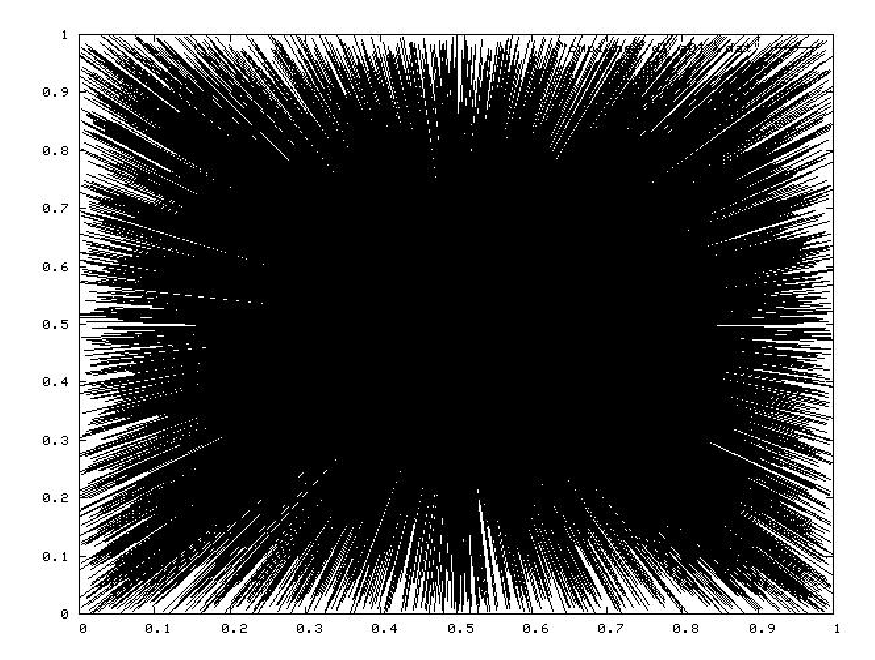
\includegraphics[scale=0.6]{pic_alfa01.eps}
\end{center}
\caption{Topology with $\alpha$ 0.1\label{t01figure}}
\end{figure}


The degree distribution related to the generated star topology 
(Figure~\ref{t01figure}) is not 
shown (it is simply a straight line).
Clearly the plots show that there is not any evidence about in-degree 
power-law distribution; only in the case of $\alpha = 4$, the corresponding 
plot exhibits a power-law like behavior at least for a subset of the nodes, 
but this is very different from what first listed paper was talking about.

\begin{figure}
\begin{center}
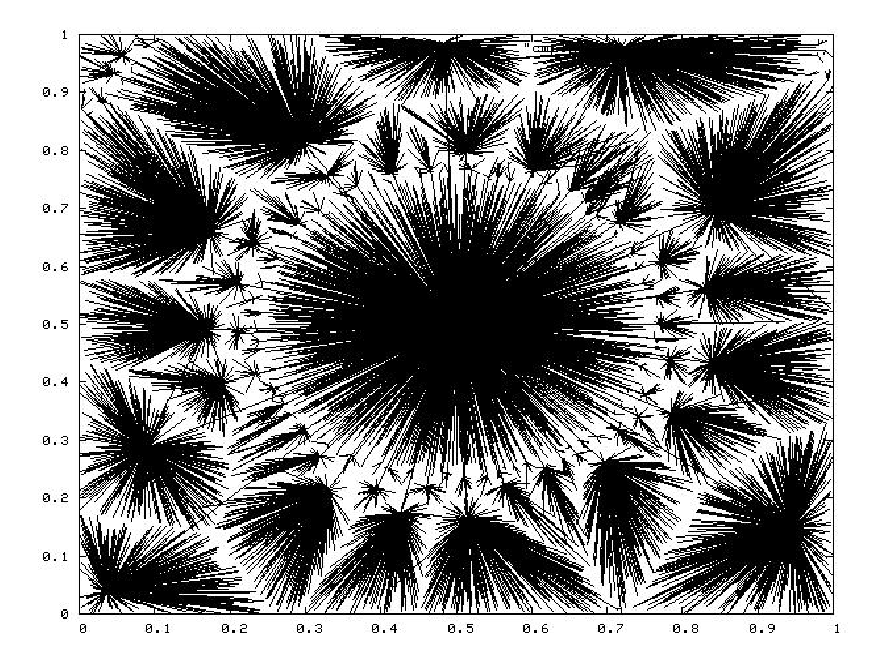
\includegraphics[scale=0.6]{pic_alfa4.eps}
\end{center}
\caption{Topology with $\alpha$ 4\label{t4figure}}
\end{figure}

\begin{figure}
\begin{center}
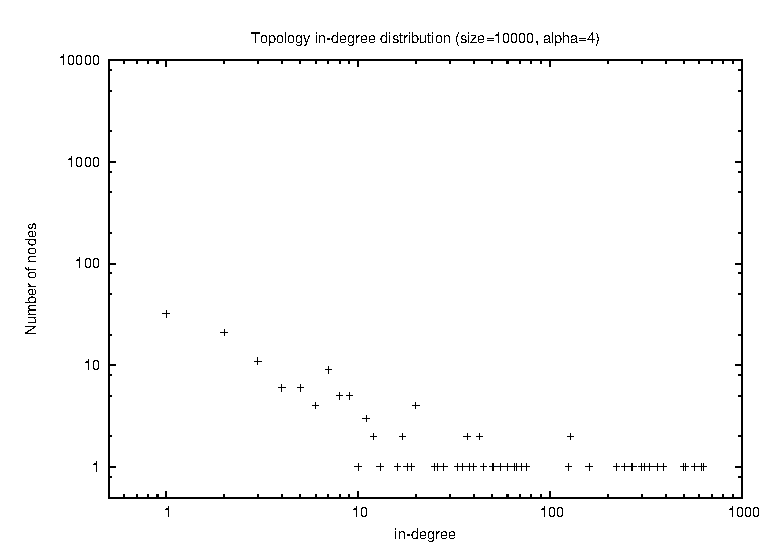
\includegraphics[scale=0.6]{picdegree_alfa4.eps}
\end{center}
\caption{In-degree distribution with $\alpha$ 4 \label{d4figure}}
\end{figure}

\begin{figure}
\begin{center}
\includegraphics[scale=0.6]{pic_alfa20.eps}
\end{center}
\caption{Topology with $\alpha$ 20\label{t20figure}}
\end{figure}

\begin{figure}
\begin{center}
\includegraphics[scale=0.6]{picdegree_alfa20.eps}
\end{center}
\caption{In-degree distribution with $\alpha$ 20 \label{d20figure}}
\end{figure}

\begin{figure}
\begin{center}
\includegraphics[scale=0.6]{pic_alfa100.eps}
\end{center}
\caption{Topology with $\alpha$ 100\label{t100figure}}
\end{figure}

\begin{figure}
\begin{center}
\includegraphics[scale=0.6]{picdegree_alfa100.eps}
\end{center}
\caption{In-degree distribution with $\alpha$ 100\label{d100figure}}
\end{figure}

\begin{figure}
\begin{center}
\includegraphics[scale=0.6]{pic_alfa2000.eps}
\end{center}
\caption{Topology with $\alpha$ 2000\label{t2000figure}}
\end{figure}

\begin{figure}
\begin{center}
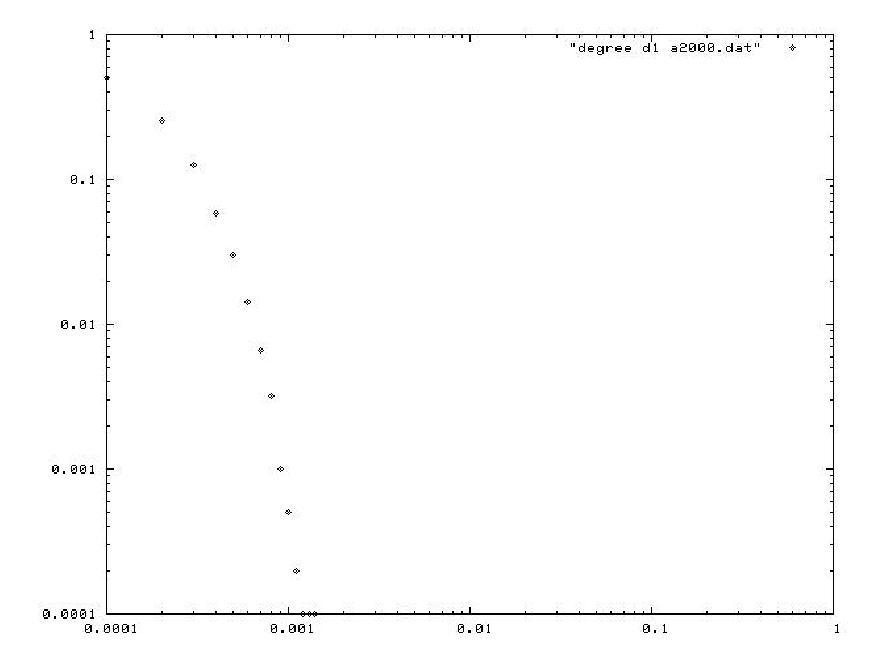
\includegraphics[scale=0.6]{picdegree_alfa2000.eps}
\end{center}
\caption{In-degree distribution with $\alpha$ 2000\label{d2000figure}}
\end{figure}

\end{document}
